\begin{frame}{Virtual Twins of Hypersonic Systems}
    \footnotesize
    \begin{columns}
        \begin{column}{0.6\linewidth}
            \centering
            \only<2>{
                \begin{figure}
                    \centering
                    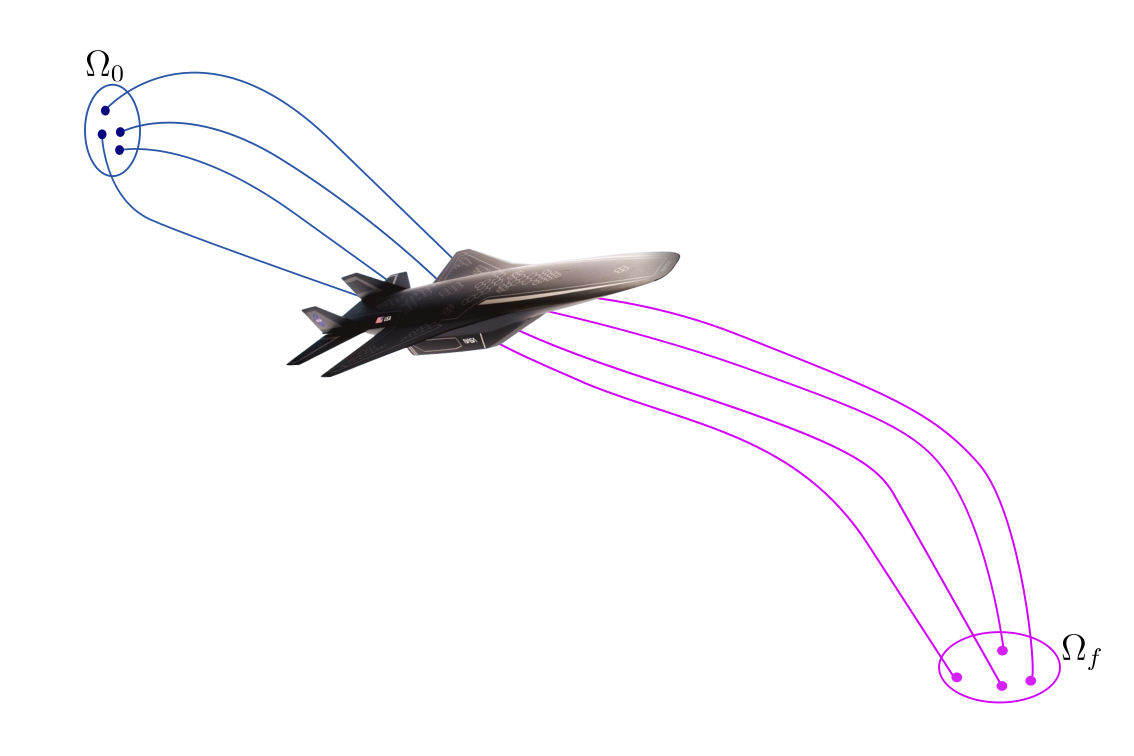
\includegraphics[width=0.9\textwidth]{../figs/introduction/motivating_example_1.png}
                \end{figure}}
            \only<3>{
                \begin{figure}
                    \centering
                    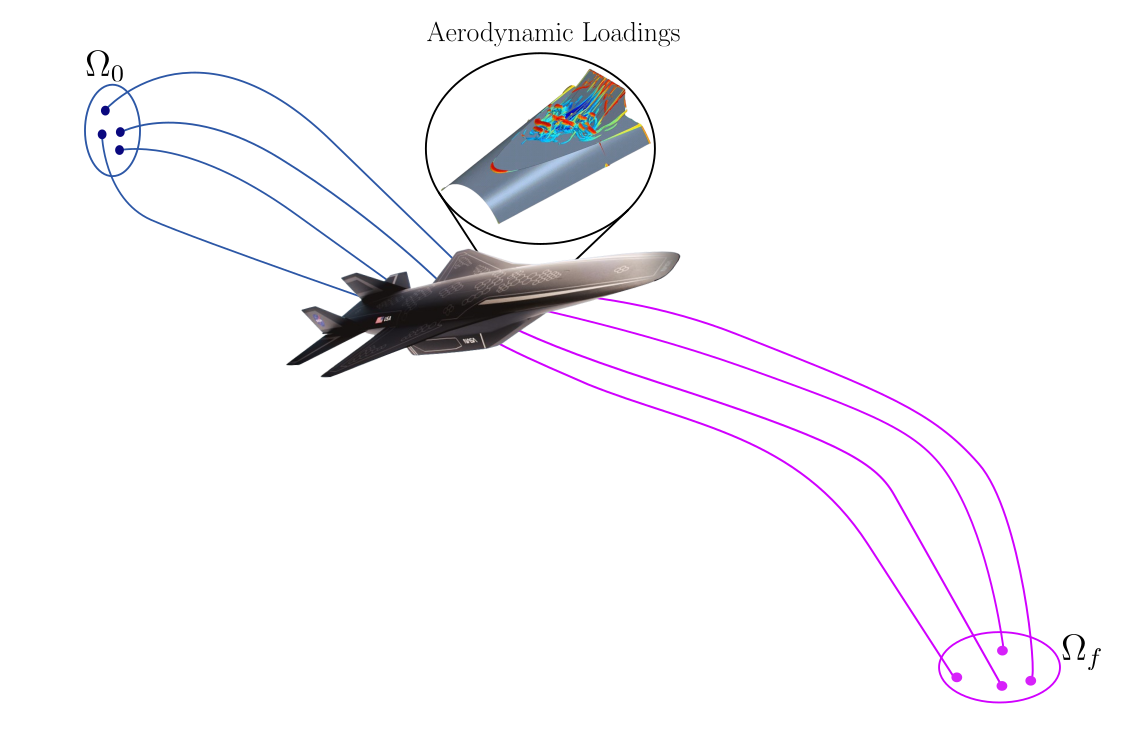
\includegraphics[width=0.9\textwidth]{../figs/introduction/motivating_example_2.png}
                \end{figure}}
            \only<4>{
                \begin{figure}
                    \centering
                    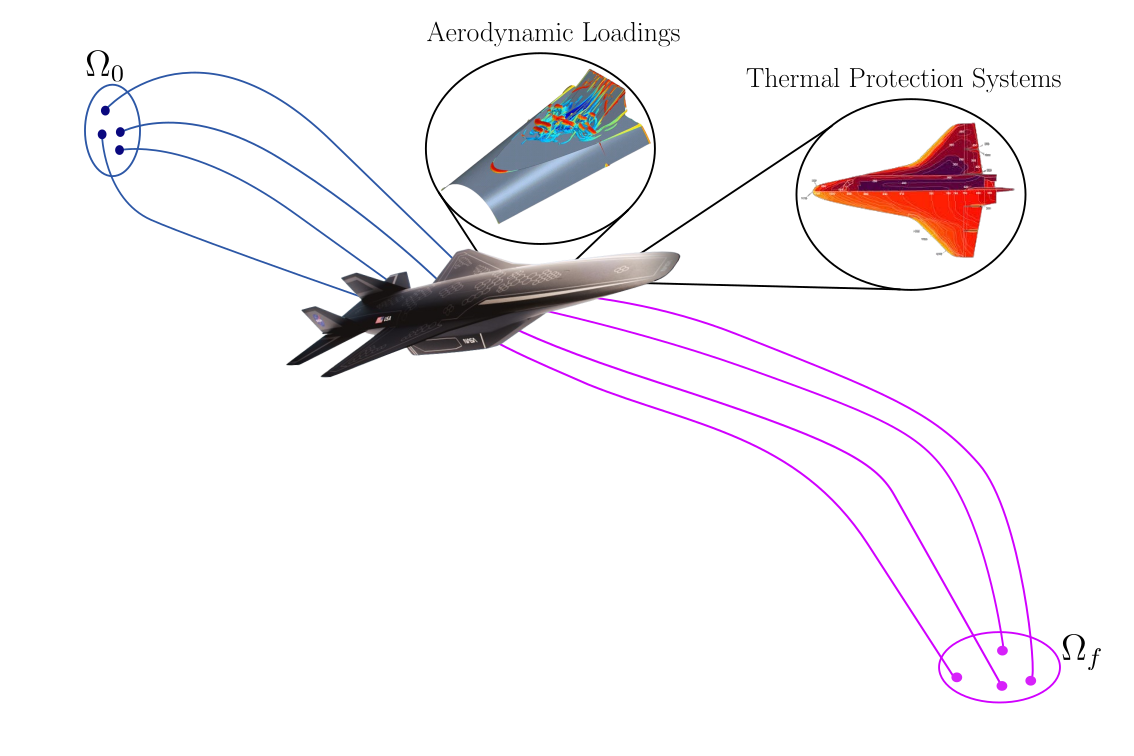
\includegraphics[width=0.9\textwidth]{../figs/introduction/motivating_example_3.png}
                \end{figure}}
            \only<5>{
                \begin{figure}
                    \centering
                    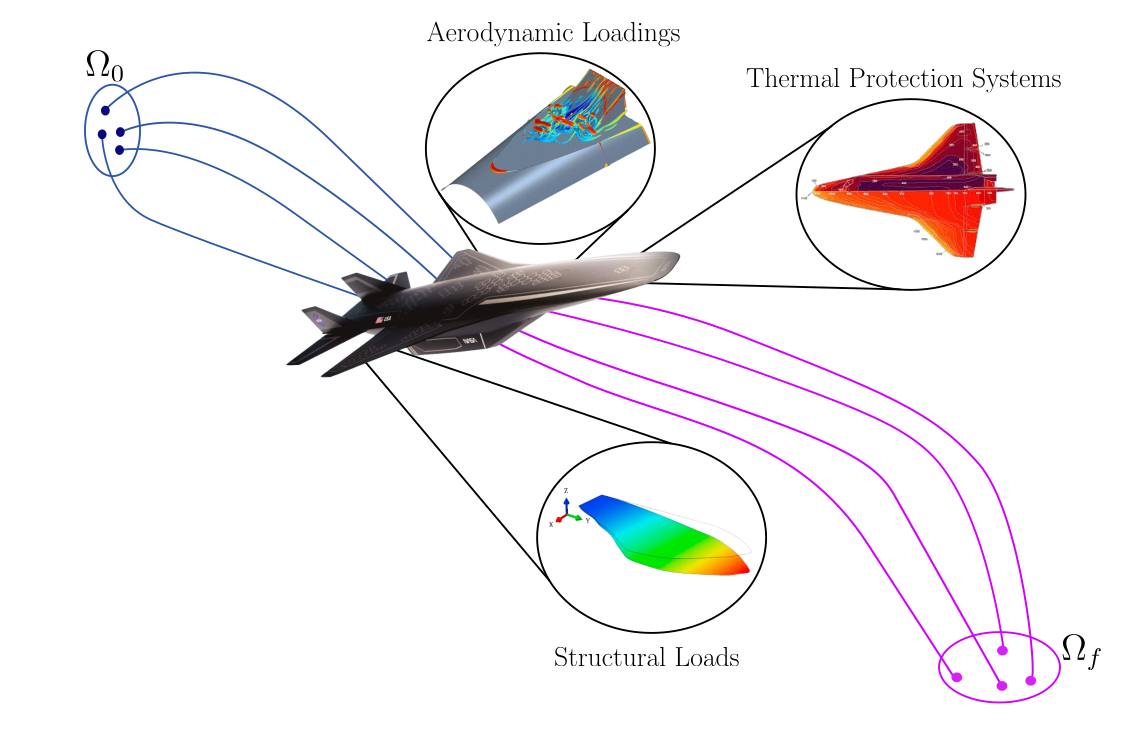
\includegraphics[width=0.9\textwidth]{../figs/introduction/motivating_example_4.png}
                \end{figure}}
            \only<6->{
                \begin{figure}
                    \centering
                    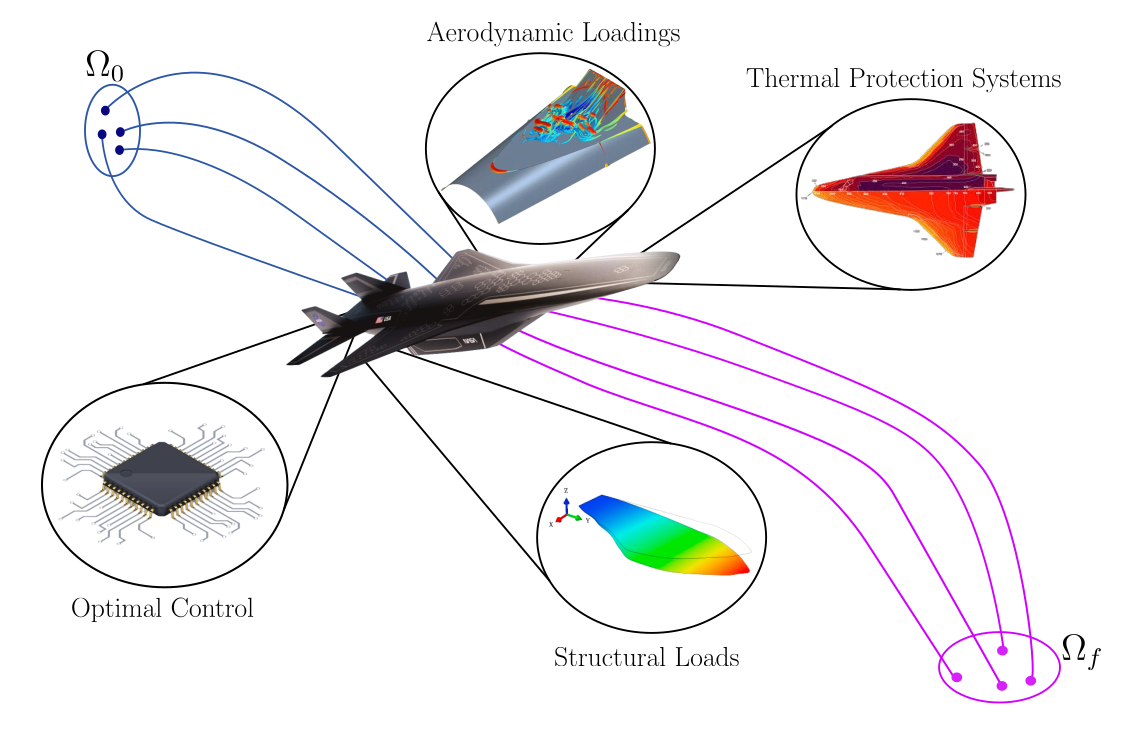
\includegraphics[width=0.9\textwidth]{../figs/introduction/motivating_example_5.png}
                \end{figure}}
        \end{column}
        \hspace*{-1in}
        \begin{column}{0.49\linewidth}
            \centering
            \visible<7-10>{
            \textbf{Finite-Element Model (FEM)}
            \begin{align*}
                \visible<8->{
                \dot{\vu} &= \mathbf{F}\left(\vu;\mathbf{p}\right)}\\
                \visible<9->{
                \vz_{\text{HF}} &= \mathbf{H}\left(\vu;\vp\right)}\\
                \visible<10->{
                \vu(t_0) &= \vu_0(\vp)}
            \end{align*}
            }
            \visible<11-14>{
            \textbf{Optimal Control Problem (OCP)}
            \begin{align*}
                \visible<12->{
                \min_{\vp} \: \mathcal{J} = \int_{t_0}^{t_f} & \ell\left(\vu,\mathbf{p}\right) dt}\\
                \visible<13->{
                \text{s.t.} \: \quad \dot{\vu} &= \mathbf{F}\left(\vu;\mathbf{p}\right)}\\
                \visible<14->{
                \mathbf{Q} &\geq \mathbf{g}\left(\vu(t),t;\mathbf{p}\right)}
            \end{align*}
            }
        \end{column}
    \end{columns}
    \visible<2->{
    \begin{center}
        {\tiny
        $\vu$: high-dimensional states, $\vF$: non-linear dynamics $\vp$: design/control parameters, $\vz_{\text{HF}}$: high-fidelity outputs, $\mathcal{J}$: cost functional, $l$: running cost, $\mathbf{Q}$: safety bound, $\vg$: constraint function}
    \end{center}}
\end{frame}

\begin{frame}{Exploration of Design Space is Costly}
    \footnotesize
    \hspace*{-0.1in}
    \only<1>{
        \begin{figure}
            \centering
            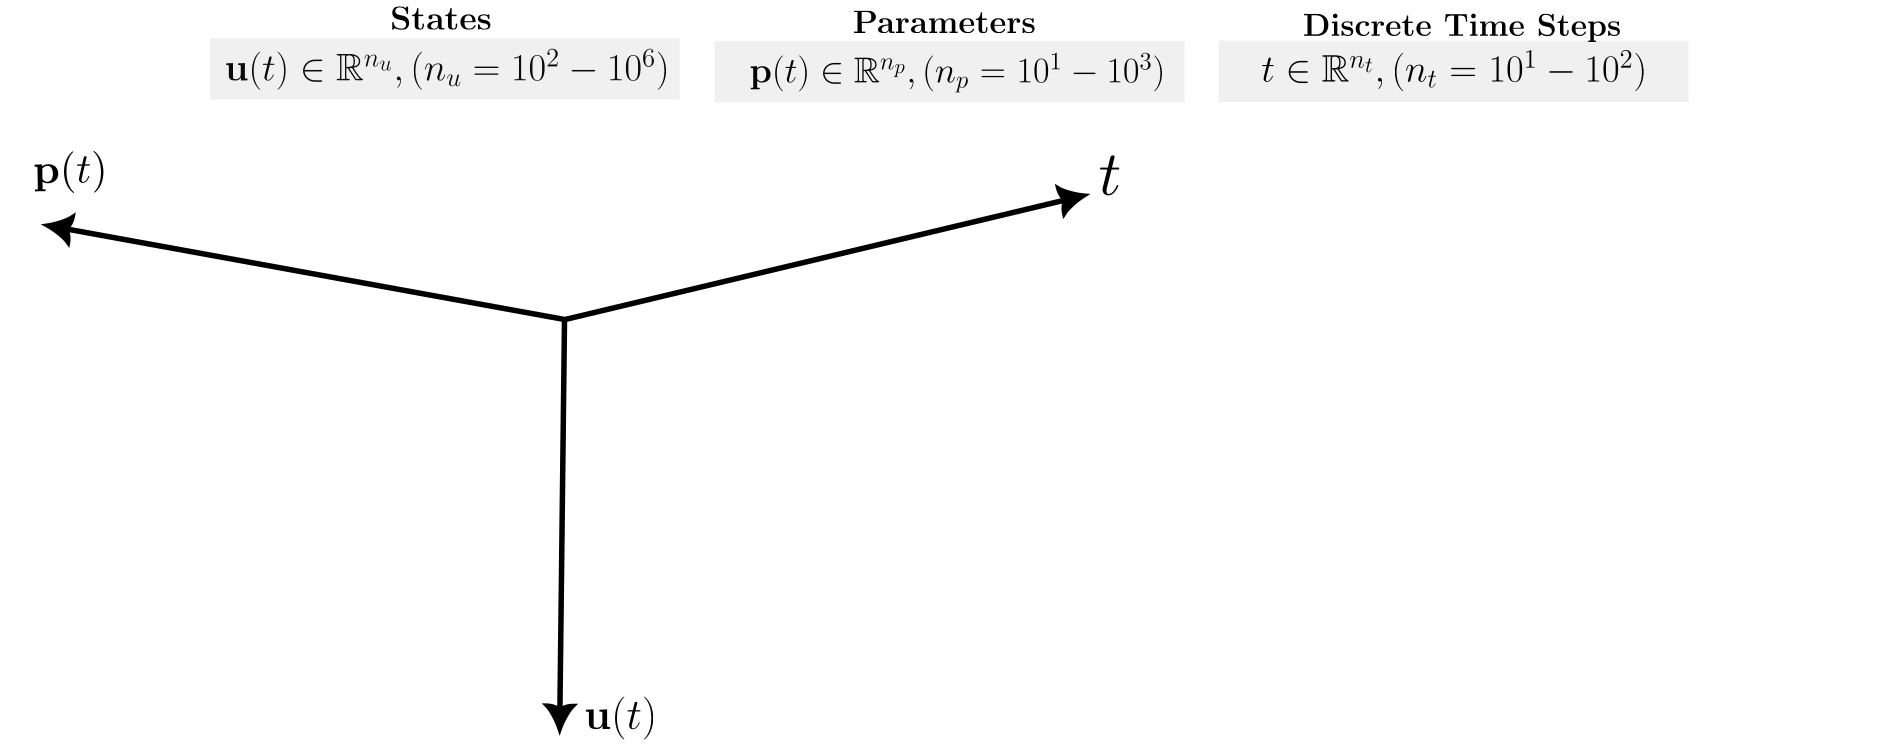
\includegraphics[width=0.95\textwidth]{../figs/introduction/problem_space_1.png}
        \end{figure}}
    \only<2>{
        \begin{figure}
            \centering
            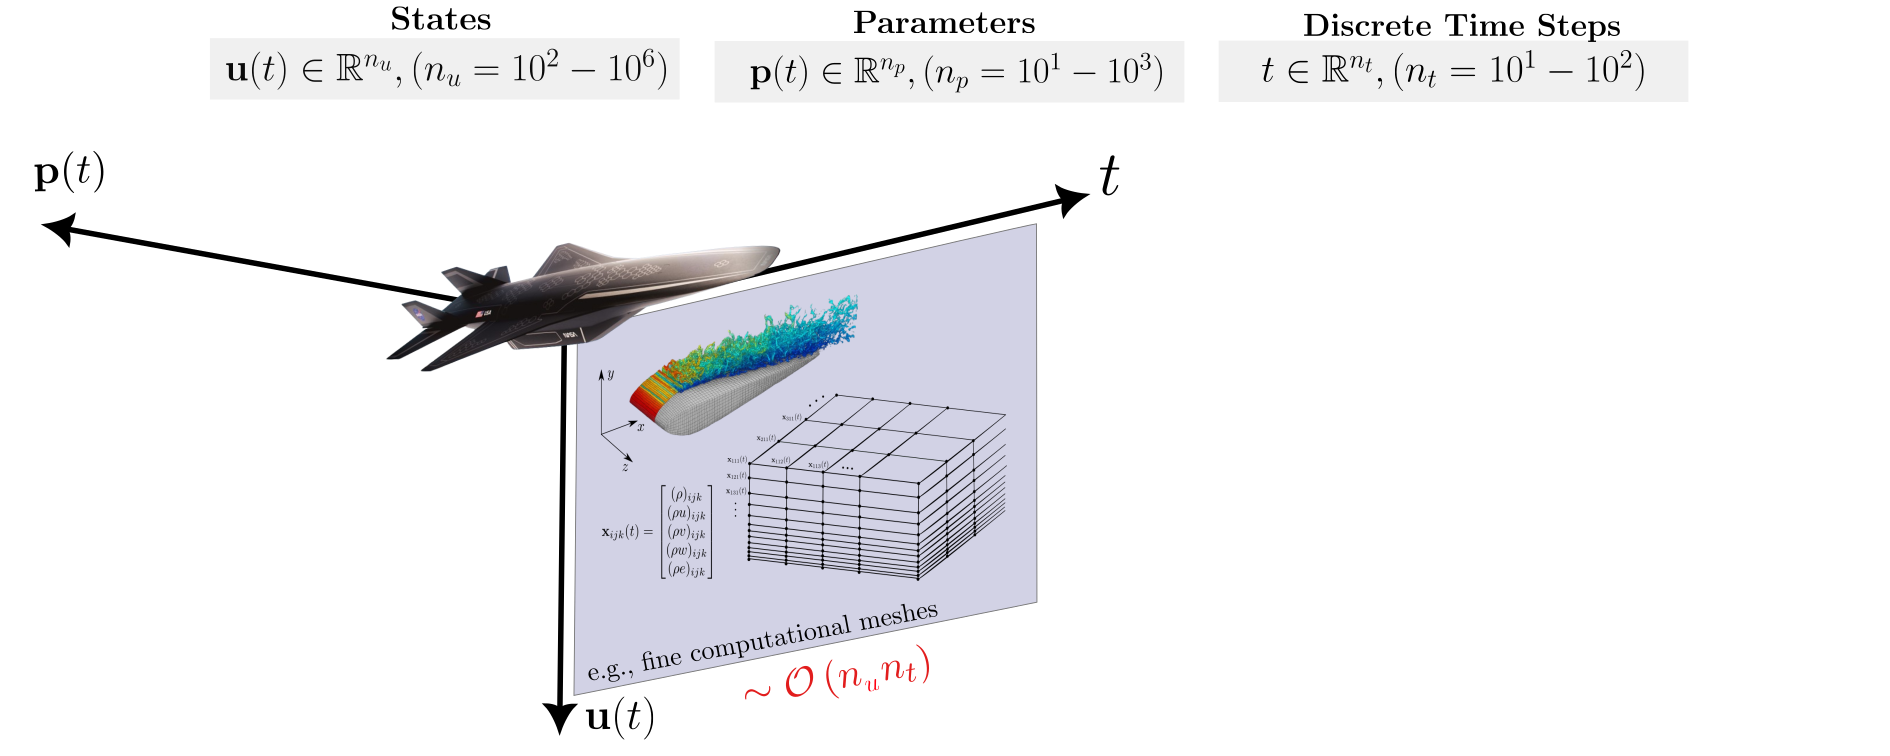
\includegraphics[width=0.95\textwidth]{../figs/introduction/problem_space_2.png}
        \end{figure}}
    \only<3>{
        \begin{figure}
            \centering
            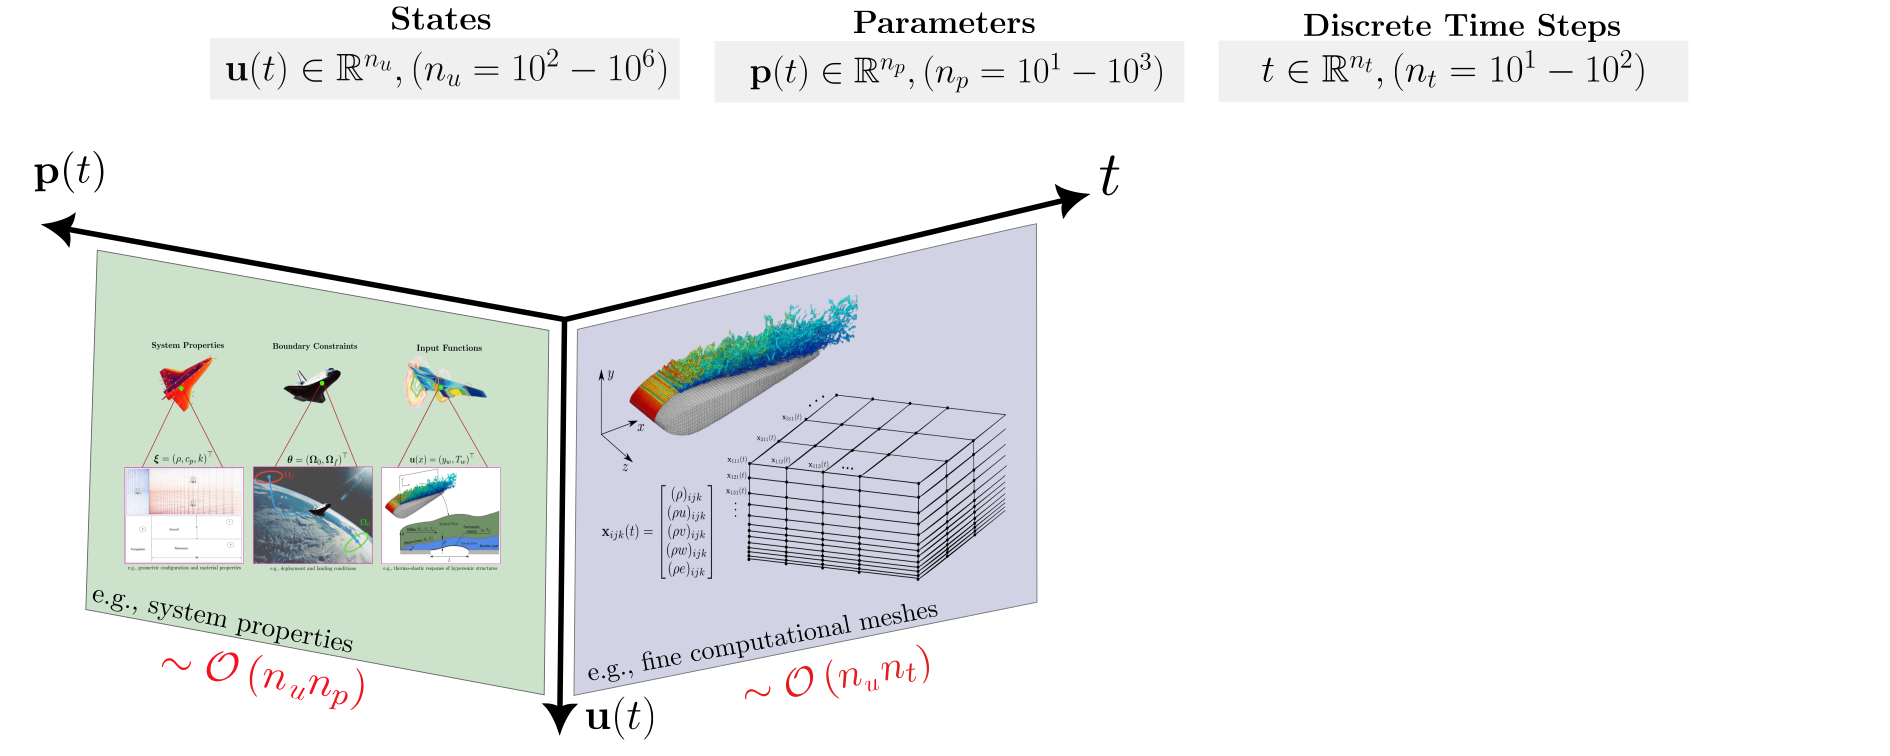
\includegraphics[width=0.95\textwidth]{../figs/introduction/problem_space_3.png}
        \end{figure}}
    \only<4>{
        \begin{figure}
            \centering
            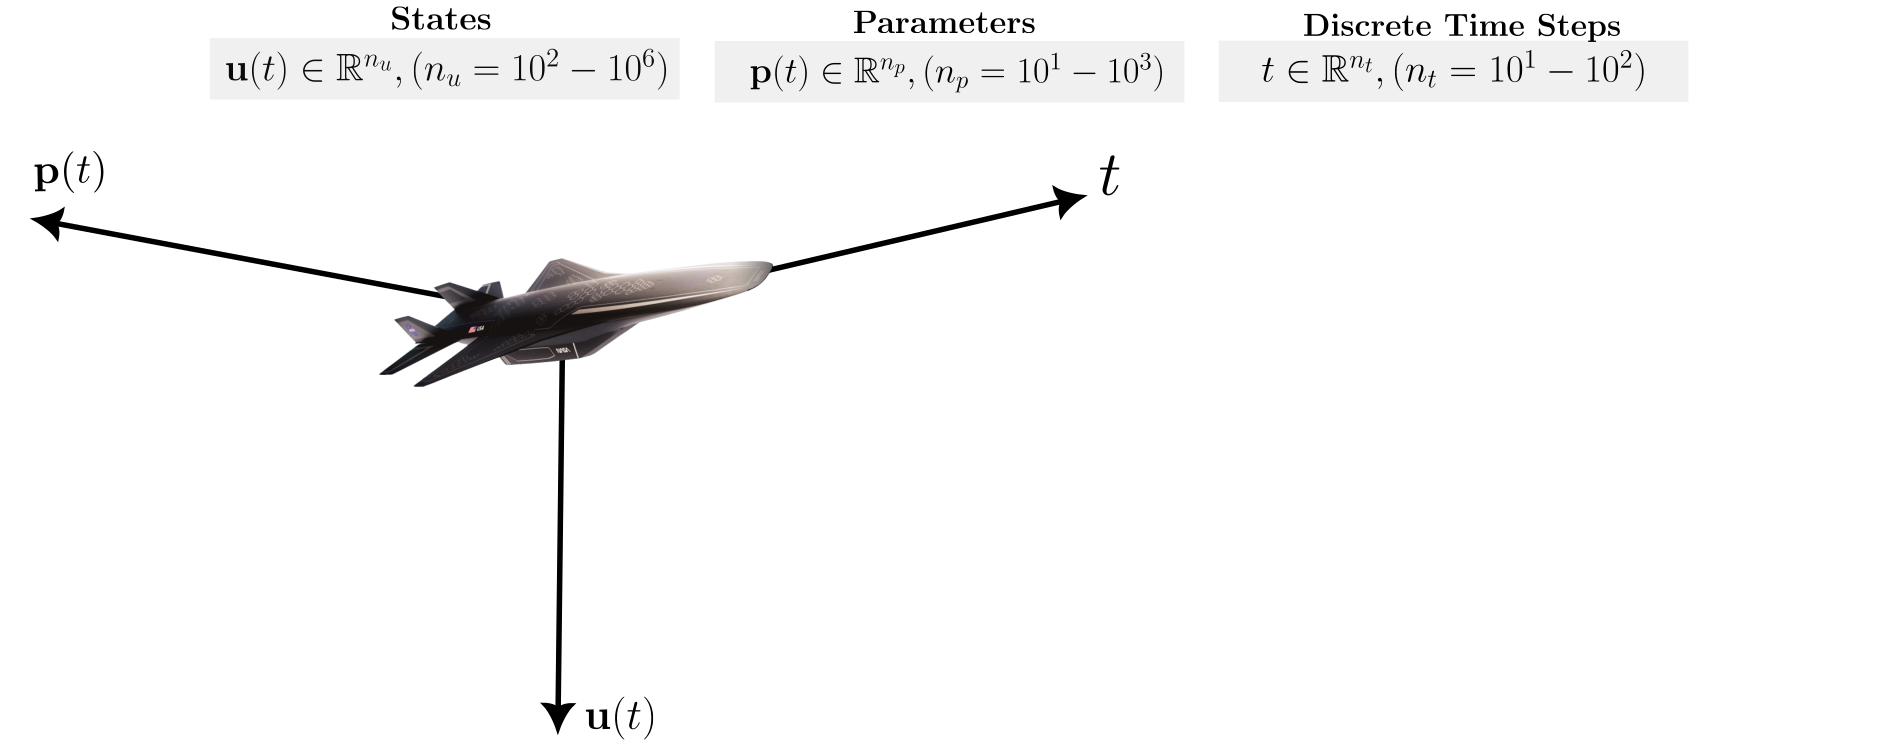
\includegraphics[width=0.95\textwidth]{../figs/introduction/problem_space_4.png}
        \end{figure}}
    \only<5>{
        \begin{figure}
            \centering
            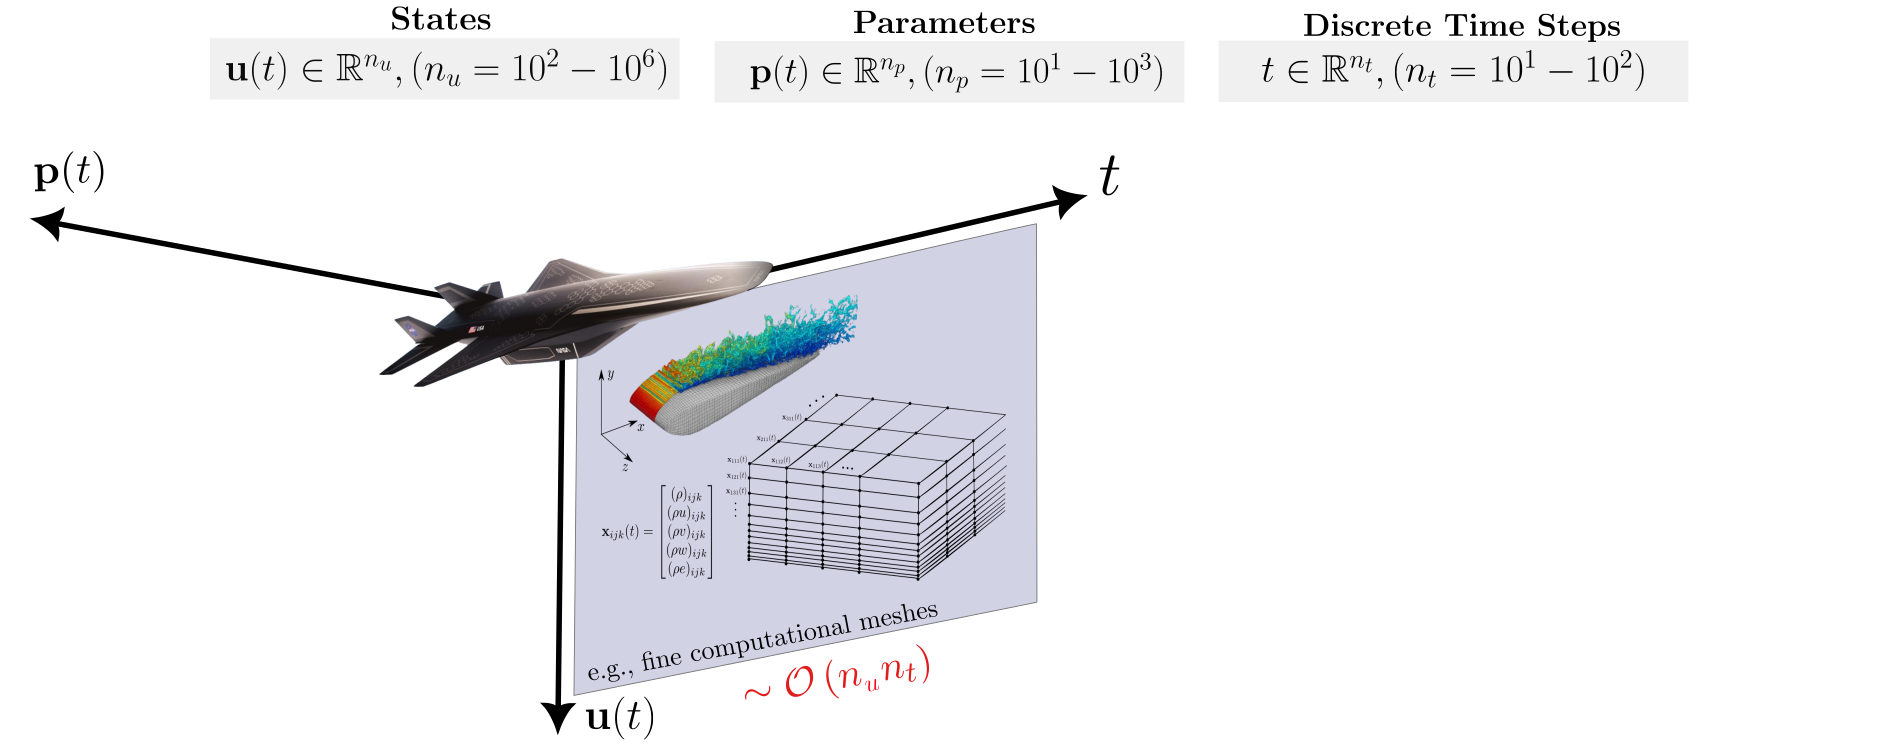
\includegraphics[width=0.95\textwidth]{../figs/introduction/problem_space_5.png}
        \end{figure}}
    \only<6>{
        \begin{figure}
            \centering
            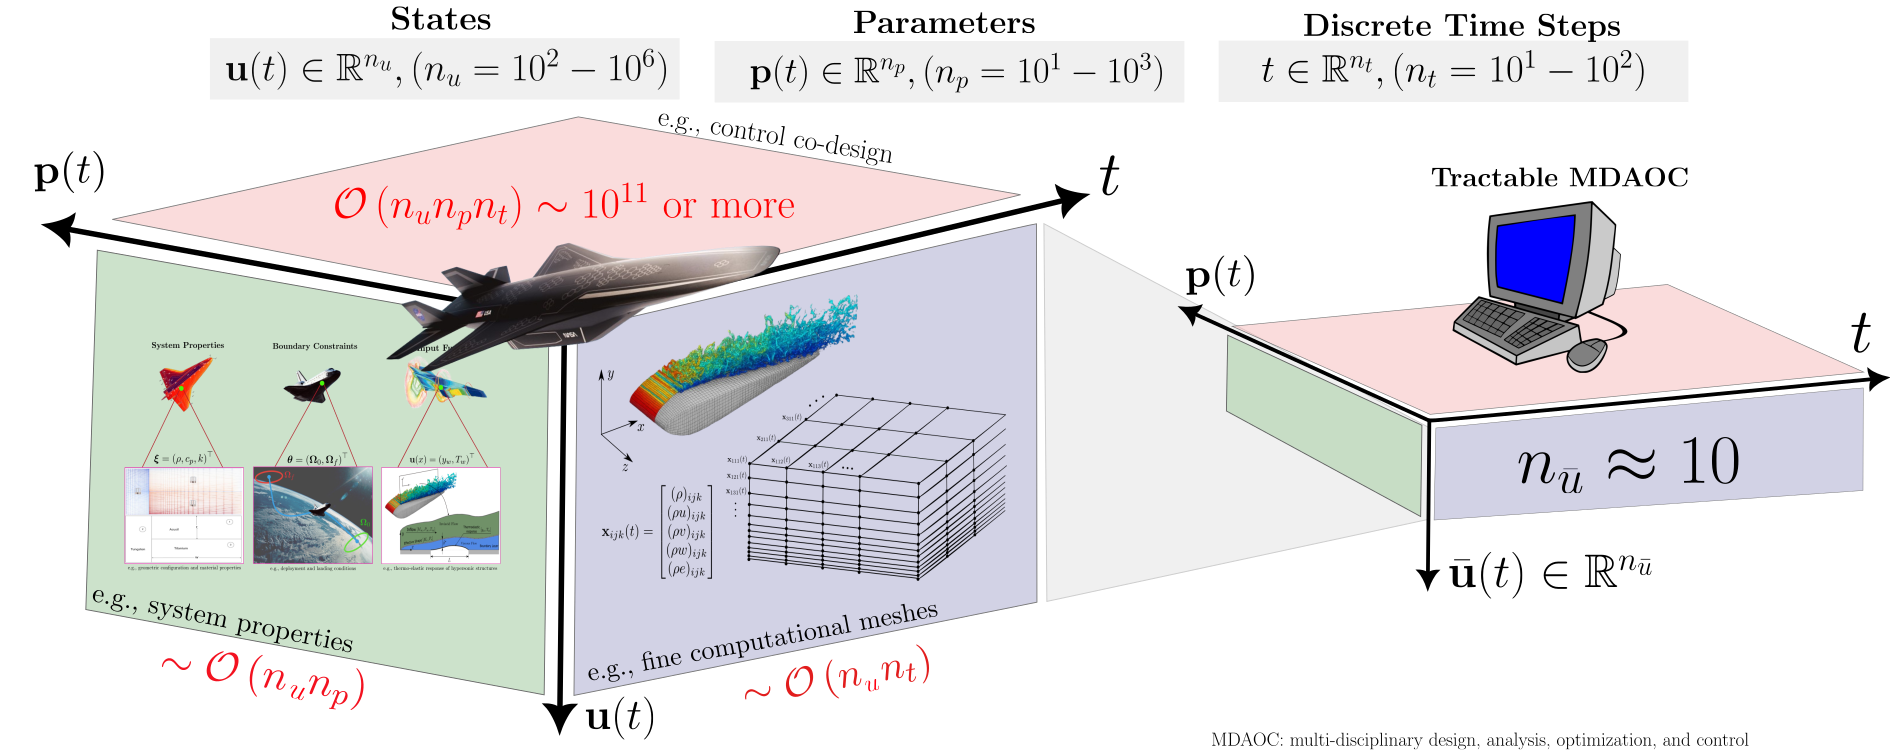
\includegraphics[width=0.95\textwidth]{../figs/introduction/problem_space_6.png}
        \end{figure}}
    \only<7->{
        \begin{figure}
            \centering
            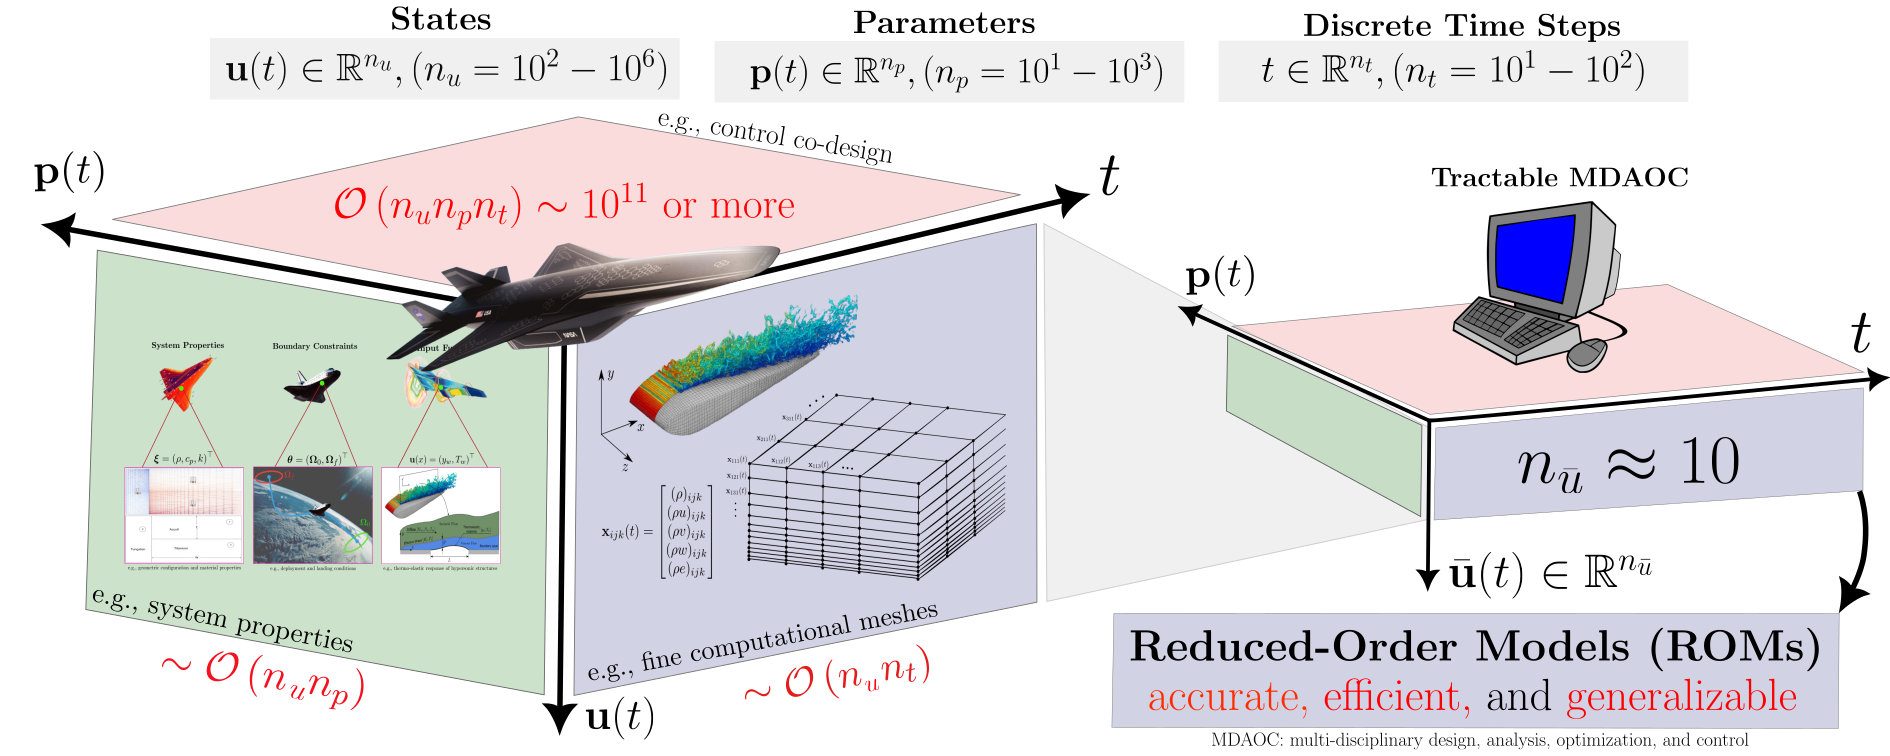
\includegraphics[width=0.95\textwidth]{../figs/introduction/problem_space_7.png}
        \end{figure}}
\end{frame}